\documentclass[a4paper, 11pt]{article}

\usepackage[czech]{babel}
\usepackage[utf8]{inputenc}
\usepackage[left=2cm, top=3cm, text={17cm, 24cm}]{geometry}
\usepackage{times}
\usepackage[unicode]{hyperref}
\usepackage{indentfirst}
\usepackage{graphics}
\usepackage{fancyvrb}
\usepackage{listings}
\usepackage{xcolor}
\lstset{basicstyle=\footnotesize\ttfamily,breaklines=true}
\lstset{framextopmargin=50pt,frame=none}
\hypersetup{colorlinks = true, hypertexnames = false}

\renewcommand*\contentsname{Obsah}

\begin{document}

	\begin{titlepage}
		\begin{center}
			\LARGE\textsc{Vysoké učení technické v~Brně} \\
			\Large\textsc{Fakulta informačních technologií}\\
			\vspace{\stretch{0.382}}
			\large{IFJ - Projektová dokumentace} \\
			\LARGE{Implementace překladače jazyka IFJ22} \\
			\vspace{0.2cm}
			\large{Tým "Tým xkalis03", varianta BVS}
			\vspace{\stretch{0.618}}
		\end{center}

		\Large{\hspace*{-0.6cm}Autoři: \hfill (v) \hspace{0.1cm} Vojtěch Kališ (xkalis03)} \hspace{0.97cm} 25\% \\
		\Large{\hspace*{\fill} Jan Lutonský (xluton02)} \hspace{0.82cm} 25\% \\
		\Large{\hspace*{\fill} Jan Salaš (xsalas02)} \hspace{1.73cm} 25\% \\
		\Large{\hspace*{\fill} Lucie Hlaváčová (xhlava60)} \hspace{0.1cm} 25\% \\ \\
		\Large{Implementovaná rozšíření:  \hspace*{1cm} FUNEXP} \hfill
	\end{titlepage}

%%% TOC
	\tableofcontents

%%%
	\newpage
	\section{Úvod}
	Cílem tohoto projektu bylo vytvořit překladač implementovaný v~jazyce C, který ze standartního vstupu načte vstupní kód napsaný v~jazyce IFJ22, přeloží
	jej do cílového jazyka IFJcode22 a výskedek pak vypíše na standartní výstup. Jazyk IFJ22 vznikl jako obdoba jazyka PHP. 
%%%
	\section{Implementace}
	Celý překladač jsme si rozdělili na více dílčích problémů, jejichž funkčnost byla individuálně testována. Tyhle dílčí problémy byly nadále vzájemně 
	propojovány a opět testována jejich funkčnost.
		\subsection{Lexikální analyzátor}
	Lexikální analyzátor jsme implementovali jako deterministický konečný automat. Z důvodu přehlednosti jsme se rozhododli jednotlivé stavy implementovat 
	jako funkce, namísto vnořených $switch$ příkazů. Lexikální analyzátor pracuje ve třech módech:
	
	\begin{itemize}
		\item \hyperref[lex_START]{START}\newline
			V tomto stavu se analyzátor snaží načítat token prologu $<?php$. Po načtení se přesune do stavu CONTINUE. Pokud v tomto módu nalezne 
			cokoliv jiného, jedná se o lexikální chybu.
		\item \hyperref[lex_CONTINUE]{CONTINUE}\newline
			V tomto stavu se analyzátor snaží zjistit, zda se po prologu nachází speciální token $declare(strict \textunderscore types=1);$. Pokud ano, 
			zpracuje jej jako validní token, jinak se přesouvá do stavu NORMAL.
		\item \hyperref[lex_NORMAL]{NORMAL}\newline
			V tomto stavu se analyzátor snaží načítat všechny ostatní tokeny. V případě, že se aktuální vstup neshoduje s žádným z definovaných tokenů, 
			jedná se o lexikální chybu.
	\end{itemize}
	
	Na začátku programu se lexikální analyzátor inicializuje funkcí $lex \textunderscore init$. Ta rovnou načte první token ze vstupu a vrátí jej syntaktickému 
	analyzátoru. Pro získání dalšího tokenu syntaktický analyzátor zavolá funkci $lex \textunderscore next$.
	\subsection{Syntaktický analyzátor}
	Syntaktický analyzátor je závislý na lexikalním; volá jeho funkce aby získal nový token. Tokeny jsou předávány přes strukturu \hyperref[cont]{context}, která 
	slouží pro sdílení dat mezi částmi překladače. Pro implementaci syntaktické analýzy byla zvolena metoda rekurzivního sestupu. Při návrhu gramatiky jsme 
	narazili na problém, kdy pravidlo pro příkaz přiřazení výrazu do proměné kolidovalo s výrazem bez přizazení, který osahuje pouze identifikátor, a z tohoto 
	důvodu jsme se rozhodli přemístit syntaktickou analýzu příkazu přiřazení do precedenční syntaktické analýzy. Další problém pak byl ještě nalezen při volání 
	funkcí, kde, z důvodu našeho rozhodnutí implementovat rozšíření FUNEXP, bylo potřeba zajistit možnost analyzovat funkce i uprostřed výrazů a jelikož nám 
	přišlo složité přepínat mezi syntaktickou analýzou rekurzivním sestupem a syntaktickou analýzou precedenční tabulkou, tak jsme se rozhodli přemístit volání 
	funkce jen do syntaktické analýzi precedenční tabulkou. Analyzátor při své funkci tvoří \hyperref[abstrtree]{abstraktní syntaktický strom}, který je dále 
	zpracováván dalšími částmi překladače.

	\subsubsection{Precedenční syntaktický analyzátor}
	Slouží ke zpracování výrazů, přikazu přiřazení do proměné a volání funkce. Při tvorbě precedenční tabulky bylo zpozorováno, že operátory je možné sjednotit 
	do množin se stejnou precedencí, díky čemuž bylo možné tabulku zmenšit. Precedenční analyzátor analyzuje vstupní tokeny získané z lexikálního analyzátoru 
	přes strukturu context, dokud nenarazí na první token, který se nesmí vyskytovat ve výrazu, volání funkce nebo v příkazu přiřazení. Tento token není 
	zkonzumován a je ponechán v struktuře context pro další zpracování syntaktickým analyzátorem metodou rekurzivního sestupu. Redukce gramatických
	pravidel na zásobníku precedenční syntaktycké analýzy probíhají pomocí stavového automatu posaném diagramem na konci 
	dokumentu.

	\subsection{Sémantický analyzátor}
	\label{semantic}
	Sémantický analyzátor provádí sémantickou analýzu nad vstupním programem, a je obsažen v souboru \textit{semantic\.c}; jeho hlavičkový soubor pak 
	analogicky nese název \textit{semantic\.h}. Sémantický analyzátor pracuje převážně s \textit{globální tabulkou symbolů} (využívající implementace 
	\hyperref[symtab]{tabulky symbolů} a \hyperref[abstrtree]{abstraktním syntaktickým stromem} (dále jen ASS); obojí se nachází ve sdílené struktuře 
	\hyperref[cont]{Context}. Očekává se korektní naplnění ASS v rámci 
	syntaktické analýzy. Na začátku své funkce sémantický analyzátor projde ASS a vyhledá v něm všechny definice funkcí, jež vloží jakožto nody s typem 	
	\textit{function} do globální tabulky symbolů; možné parametry definované při deklaraci funkce zase vloží do \textit{lokální tabulky symbolů} dané funkce 
	jakožto nody s typem \textit{variable}. Do globální tabulky symbolů jsou také vloženy deklarace vestavěných funkcí (zavoláním funkce ), společně s funkcí 
	nazvanou ":b" sloužící jako hlavní tělo programu (\textit{body}).

	Jakmile je vše připraveno, Sémantický analyzátor vstoupí do funkce \textit{AST\_DF\_traversal}, plnící funkci hlavní smyčky, která prochází již zmíněný AST 
	do hloubky a v rámci switch case-u pak hledá AST nody, jejichž sémantickou korektnost je třeba prověřit; jakmile nějakou takovou nodu najde, spustí nad ní 
	speciální funkci zabývající se prověřením sémantické korektnosti toho konkrétního typu AST nody. V případě, že je nalezena sémantická chyba, program 
	ukončí svou činnost, vypropaguje kód odpovídající nalezené chybě, a zaručí, že dojde ke kompletnímu uvolnění veškeré alokované paměti.
	\subsection{Generátor cílového kódu}
	Na začátku programu jsou definovány globální proměné a lokální proměné na hodnotu nill. Dále následuje hlavní telo programu. Na konci jsou vygenerovány 
	všechny vestavěné funkce.
	\subsubsection{Definice funkcí}
	Při vstupu do funkce se vytvoří nový lokální rámec, do něž se přesunou parametry volané funkce z datového zásobníku, a následně jsou inicializovány 
	všechny lokální proměné v lokálním rámci na nil. Na konci funkce se na datový zásobník vloží návratová hodnota funkce a to i v případě funkcí vracejících 
	void, v tomto případě se vrací nil.
	\subsubsection{Volání funkcí}
	Při volání funkce se na datový zásobní vloží všechny parametry volané funkce zprava do leva, a pokud se jedná o vestavěnou funkci write (jediná variadická 
	funkce) je nakonec na datový zásobník vložen i počet předaných parametrů funkce. Při návratu z funkce je návratová hodnota ponechána na datovém 
	zásobníku pro dalši zpracování.
	\subsubsection{Výrazy}
	Výrazy jsou vyhodnovocány převážne za použití datového zásobníku. Při generování výrazů jsou prováděny dynamické typové konverze podle tabulky ze 
	zadání.
%%%
	\section{Speciální datové struktury}
	\subsection{Context}
	\label{cont}
	Jedná se o strukturu určenou pro sdílení dat mezi lexikálním analyzátorem, syntaktickým analyzátorem, sémantickým analyzátorem i generátorem cílového 
	kódu. Obsahuje globální tabulku symbolů, buffed posledního tokenu, buffer atributu posledního tokenu (jeho přímá "stringová reprezentace"), kořen AST a 
	zásobník pro precedenční syntaktickou analýzu.
	\subsection{Abstraktní syntaktický strom}
	\label{abstrtree}
	Je implementován jako \href{https://en.wikipedia.org/wiki/M-ary_tree}{N-ární strom}. Tento strom je tvořen při syntaktické analýze a slouží jako vnitřní 
	reprazentace vstupního kódu. Abstraktní syntaktický strom je ze syntaktické analýzy předávan analýze sémantické, která jej prochází a kontroluje 
	sémantickou korektnost. Po ověření sémantickou analýzout je strom dále předán generátoru cílového kódu, který strom projde a generuje úseky kódu v 
	závislosti na uzlech stromu. N-arní strom zjednodušil zpracování zřetězených gramatických pravidel, jako například seznam parametrů při definici funkce 
	nebo seznam parametrů při volání funkce.

	\subsection{Generický zásobník}
	Je implementován pomocí dynamického pole ukazatelů na void. Při přidávání prvků na zásobník může dojít místo v dynamickém poli, v takovém případě je k 
	poli přialokováno 24 volných slotů zásobníku pomocí funkce realloc. Přialokovávání 24 položek by mělo být dostatečné, avšak nebyly podniknuty žádná 
	měření či testy které by tuhle skutečnost potrdily.
    
	\subsection{Zásobník pro precedenční syntaktickou analýzu}
	Je přetypovaná struktura generického zásobníku. Pro tento zásobník byly vytvořeny funkce, které správně přetypují vstupy a výstupy tak, aby bylo možné 
	volat funkce generického zásobníku. Samotný zásobník slouží pro ukládání uzlů syntaktického stromu, které jsou následně redukovány precedenčním 
	syntaktickým analyzátorem.

	\subsection{Tabulka symbolů}
	\label{symtab}
	Tabulka symbolů byla implementována jako binární vyhledávací strom, což bylo i nárokem naší varianty zadání. Téměř celá tabulka symbolů je napsána 
	nerekurzivním (tedy iterativním) postupem, a to především z důvodu snížení časové komplexity na úkor složitější implementace. Tabulka symbolů je 
	využívána \hyperref[semantic]{Sémantickým analyzátorem} pro vytvoření Globální tabulky symbolů a její využití je již popsáno v rámci jeho popisu.

	\subsection{Obousměrně vázaný seznam}
	Implementaci obousměrně vázaného seznamu lze najít v souboru \textit{dll.c}, a odpovídající hlavičkový soubor pak pod názvem \textit{dll.h}. Obousměrně 
	vázaný seznam je v projektu využíván ve struktuře nody Tabulky symbolů, a to pro účely snadného uchování názvů argumentů vkládaných funkcí.
%%%
	\section{Práce v týmu}
	Na projektu jsme začali pracovat ihned po zveřejnění zadání, a to jeho prostudováním a domluvením první schůzky, v rámci které byla vypracována prvotní 
	verze pravidel LL-gramatiky, a LL tabulka. Obojí se ještě v čase dalších několika týdnů upravovalo v případě nalezení chyby, až se nakonec vše ustálilo do 
	konečné podoby, prezentované v tomhle dokumentě a dohledatelné na jeho \hyperref[gram]{konci}.
	
	Dále jsme si jednotlivé části rozdělili mezi sebe a pracovali na nich jako jednotlivci popřípadě dvojice. Stále probíhaly schůzky, například pro řešení 
	implementačních záležitostí a to především způsobu komunikace jednotlivých částí překladače, ovšem zvětšiny docházelo spíše k průběžnému testování 
	překladače jako celku a kontrole pokroku ve vývoji.
	\subsection{Komunikace}
	Pro komunikaci byla využita aplikace \textit{Discord}, kde byl vytvořen vlastní server na kterém pak probíhala veškerá vzájemná komunikace, ať už se 
	jednalo o komunikaci textovou, hovorové schůzky celotýmové i třeba v menším počtu, nebo sdílení materiálů, diagramů apod. 
	\subsection{Vzdálený repozitář}
	Jako vzdálený repozitář jsme zvolili Github, jenž nám umožnil sdílet mezi sebou zdrojové kódy dílčích úkolů a~navzájem si testovat nejen funkčnost 
	jednotlivých částí, ale i~překladač jako celek.
	\subsection{Rozdělení práce v týmu}
		\hspace*{0.25cm}	Vojtěch Kališ (xkalis03): \hspace{0.2cm} Sémantická analýza, Tabulka symbolů, Speciální datové struktury,\\
		\hspace*{5.08cm} Testování, Dokumentace\\
		\hspace*{0.8cm} 	Jan Lutonský (xluton02): \hspace{0.2cm} Syntaktická analýza, Precedenční syntaktická analýza, Generátor\\
		\hspace*{5.08cm} cílového kódu, Speciální datové struktury, Testování, Dokumentace\\
		\hspace*{1.5cm}	Jan Salaš (xsalas02): \hspace{0.2cm} Lexikální analýza, Speciální datové struktury, Testování, Dokumentace\\
		\hspace*{0.25cm}	Lucie Hlaváčová (xhlava60): \hspace{0.2cm} Lexikální analýza, Speciální datové struktury, Testování, Dokumentace\\
%%%
	\section{Závěr}
	Ačkoliv byla práce na projektu započata poměrně brzy, díky jeho rozměrnosti nám i tak implementace překladače zabrala spoustu času a stála spoustu úsilí. 
	Avšak zkušenosti, získané během řešení projektu, a to nejen z hlediska programovacího, nýbrž i komunikace v týmu a rozebírání logistických problémů, 
	bere celý tým jako velice přínosné a nenahraditelné. 

	Během projektu jsme se potýkali s nesrovnalostmi v zadání či přímo chybějící specifikace některých specifik, avšak ty byly vyřešeny konzultací fóra k 
	projektu. Velice nám také pomohlo pokusné odevzdání, které nám dodale důležitou zpětnou vazbu ještě před řádným termínem odevzdání.
%%%
	\newpage
	
	\begingroup\centering
	\section*{DKA pro lexikální analyzátor}
	\endgroup
	\vspace{1.8cm}
	\begin{figure}[h]
		\centering
		\hspace*{-1.2cm}
		\scalebox{0.8}{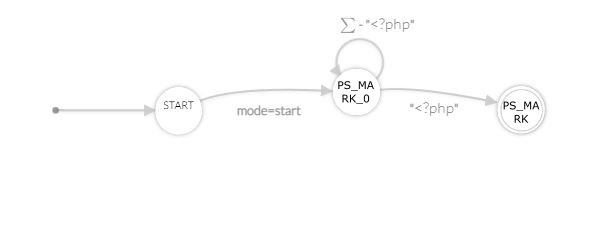
\includegraphics{diagrams/dka_start.png}}
		\label{lex_START}
		\caption{DKA pro START stav lexeru}
	\end{figure}
	\begin{figure}[h]
		\centering
		\hspace*{-1.2cm}
		\scalebox{0.6}{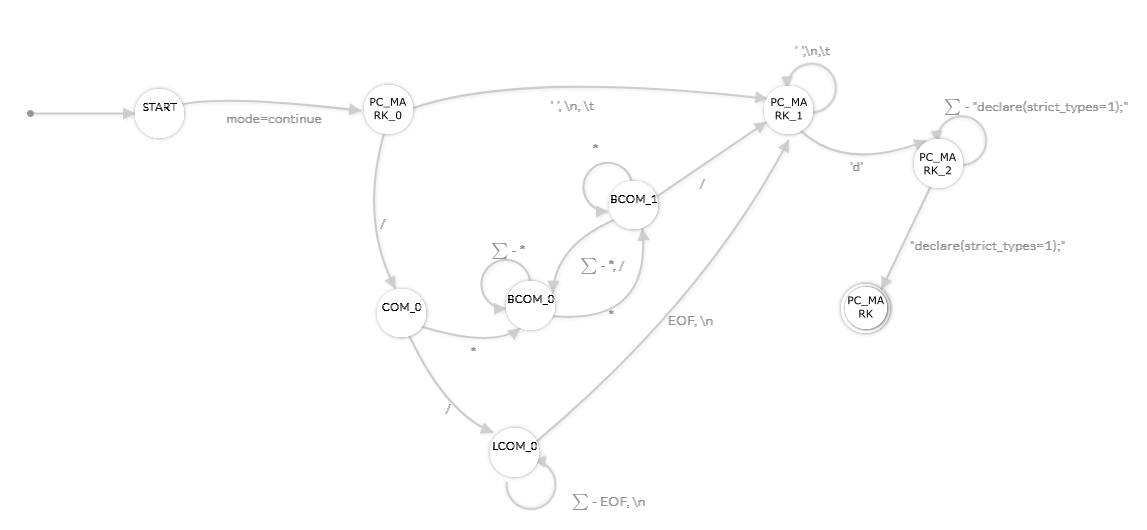
\includegraphics{diagrams/dka_continue.png}}
		\label{lex_CONTINUE}
		\caption{DKA pro CONTINUE stav lexeru}
	\end{figure}
	\begin{figure}[h]
		\centering
		\hspace*{-1.2cm}
		\scalebox{0.5}{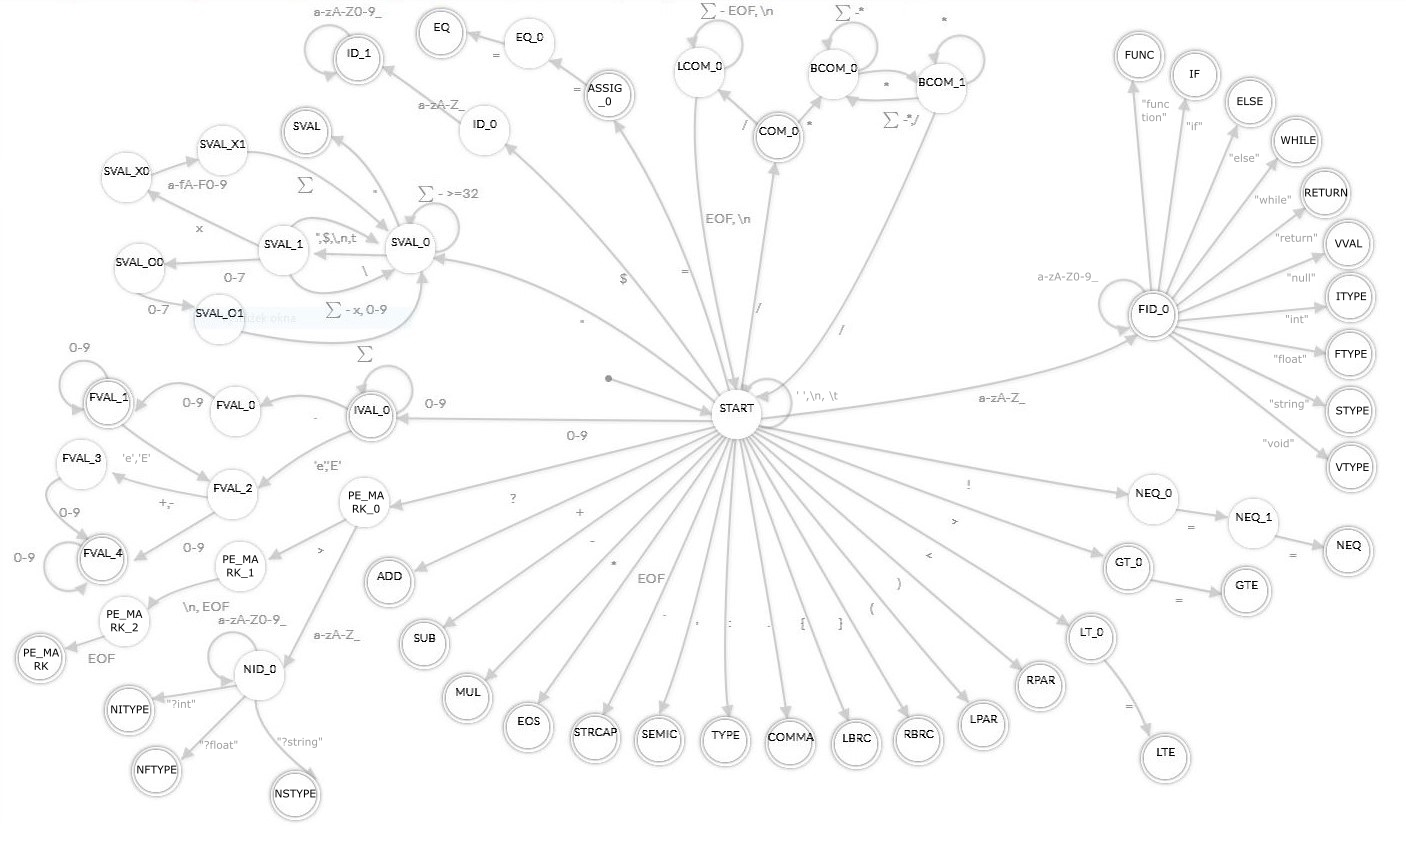
\includegraphics{diagrams/dka_normal.png}}
		\label{lex_NORMAL}
		\caption{DKA pro NORMAL stav lexeru}
	\end{figure}
%%%
	\newpage*
	\newpage*

	\begingroup\centering
	\section*{Precedenční tabulka}
	\endgroup
	\vspace{1.8cm}
	\begin{figure}[h]
		\centering
		\hspace*{-2cm}
		\scalebox{0.7}{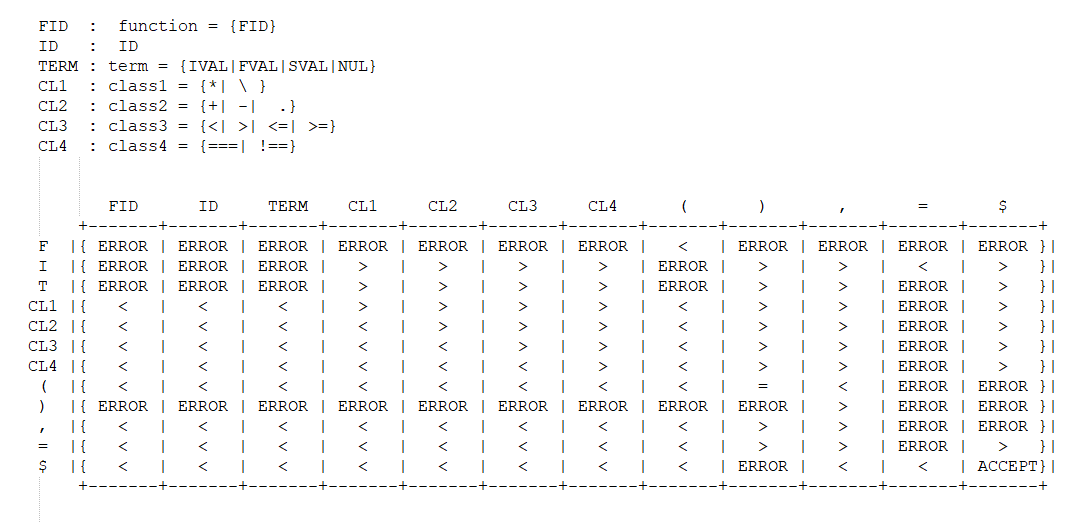
\includegraphics{diagrams/precedence_table.png}}
		\label{prec_table}
		\caption{Precedenční tabulka}
	\end{figure}
%%%
	\newpage
	
	\begingroup\centering
	\section*{Pravidla LL gramatiky}
	\label{gram}
	\endgroup
	\begin{lstlisting}[language=Python]
	prog -> PS_MARK PC_MARK prog_body

	prog_body -> body_part prog_body
	           | fun_def prog_body
	           | EPS
	
	prog_end -> PE_MARK EOS
	          | EOS
	
	body -> body_part body
	      | EPS
	
	body_part -> if_n
	           | while_n
	           | extended_expr
	           | ret
	
	extended_expr -> EXPR SEMIC 
	               | EXPR_FCALL SEMIC
	               | EXPR_PAR SEMIC
	               | EXPR_ASSIGN SEMIC
	
	ret -> RETURN ret_cont
	ret_cont -> EXPR SEMIC
	          | EXPR_PAR SEMIC
	          | EXPR_FCALL SEMIC
	          | SEMIC
	
	while_n -> WHILE EXPR_PAR LBRC body RBRC
	
	if_n -> IF EXPR_PAR LBRC body RBRC else_n
	else_n -> ELSE LBRC body RBRC
	        | EPS
		  
	fun_def -> FUNC F_ID LPAR par_list RPAR TYPE ret_type LBRC fun_body RBRC
	
	par_list -> type_n ID par_list_cont
	          | EPS
	
	par_list_cont -> COMMA par_list
	               | EPS
				
	ret_type -> type_n
	          | VTYPE
	
	type_n -> STYPE
	        | ITYPE
		| FTYPE
		| NSTYPE
		| NITYPE
		| NFTYPE

	\end{lstlisting}

%%%

\end{document}